\documentclass{article}
\usepackage{listings}
\usepackage{graphicx}
\usepackage{hyperref}
\hypersetup{pdfpagemode=Fullscreen,
  colorlinks=true,
  linkfileprefix={}}
% New conditional to allow formatting with or without extra text
\newif\ifverbose  % starts out false by default
%\verbosetrue  % remove comment to format copy with verbose comments hidden

% Page Layout
\setlength{\textheight}{\paperheight}
\addtolength{\textheight}{-2in}
\setlength{\topmargin}{-.625in}
\addtolength{\topmargin}{-.5\headheight}
\setlength{\headsep}{.375in}
\addtolength{\headsep}{-.5\headheight}
\setlength{\footskip}{.375in}
\setlength{\textwidth}{\paperwidth}
\addtolength{\textwidth}{-2in}
\setlength{\oddsidemargin}{-.5in}
\setlength{\evensidemargin}{-.5in}
\setlength{\parindent}{0pt}
\addtolength{\parskip}{3pt}


\title{EECS2502 Tutorial 3}
\date{Winter 2025}

\newcommand{\code}{\texttt}

\begin{document}

%\maketitle
\begin{center}
\begin{Large}
  \textbf{Recursion and Trees}
\end{Large}

\end{center}



\section*{Task 1: Another tree method}
In this task, you'll get another chance to practice using recursion on trees.

In the starter code, write a recursive method \verb|__eq__| that tests whether two trees are equal. Two trees are equal if and only if their root values are equal, they have the same number of subtrees, and each of the corresponding subtrees are equal - \emph{order matters}.

Note that \verb|__eq__| is another built-in Python method, and can be called either using the regular method call syntax  \verb|tree1.__eq__(tree2)|, or the more convenient syntax \verb|tree1 == tree2|.

A corner case: if \verb|tree1| is empty, then \verb|tree1 == tree2| is \verb|True| if and only if \verb|tree2| is also empty. Don't forget about this!

You may not use any other Tree methods here, other than \verb|is_empty| and helpers you defined yourself. You may access all Tree attributes.

\section*{Task 2: Nested lists and trees}
We have already noted the structural similarities between trees and nested lists in lecture. In fact, we can represent every tree as a nested list, where the first item of the nested list is the root of the tree, and each other item in the nested list is a nested list representation of one of the tree's subtrees.

For example, consider the following tree:

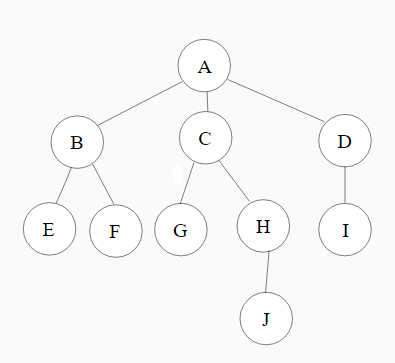
\includegraphics{tree}

Its nested list representation is

\begin{verbatim}
['A', ['B', ['E'], ['F']],
      ['C', ['G'], ['H', ['J']]],
      ['D', ['I']]]
\end{verbatim}

Note: we've done some extra whitespace formatting to make the structure clearer; you won't see this when you run the code yourself.

The nested list representation of an empty tree is simply the empty list. The nested list representation of a tree with a single item \verb|x| is \verb|[x]|.

Your task is to write a Tree method \verb|to_nested_list|, which returns a nested list representation of a tree, and the function  \verb|to_tree|, which takes a nested list and returns the Tree that it represents.

You may not use any Tree methods here other than the constructor, \verb|is_empty|, and any helpers you define yourself. You may access all Tree attributes.
\end{document}

